\section{Design \& Implementation}
\subsection{Instruction Set Extension}

The Leros microcontroller has a restricted instruction set, lacking multiply or
divide instructions, and shift and rotate operations. A multiplication
instruction was originally required for the project's selected application (a
fast Fourier transform), and therefore required a change to Leros' code. Such a
change was complicated by the structure of Leros' instruction register, which
did not have room for the additional logic to accommodate new operations. Since
the Leros code supports only two arithmetic instructions, a single bit in the
opcode was used to determine whether the instruction was an ADD or a SUB
instruction.

The first 5 bits of the instruction in the Leros CPU corresponded to that shown
in Table \ref{tab:original-instruction}.

\begin{table}
\centering
\caption{The original Leros instruction categories}
\label{tab:original-instruction}
\begin{tabular}{|l|l|}
\hline
\textbf{Bits} & Meaning \\
\hline
\texttt{00000} & NOP \\
\texttt{00001} & arithmetic operation (ADD/SUB) \\
\texttt{00010} & right shift \\
\texttt{00011} & reserved \\
\texttt{00100} & logic pperation \\
\texttt{00101} & load \\
\texttt{00110} & store \\
\texttt{00111} & IO \\
\hline
\end{tabular}
\end{table}

Whether the arithmetic instruction was an ADD or SUB was further determined by
the second bit of the instruction. It was decided that this was inefficient and
limiting. However, it was desirable that any changes to the opcode preserved the
majority of the existing form. The instruction format was changed such that the
first 5 bits of the instruction simply set a flag, and the actual operation was
encoded in bits 1 and 2 of the instruction. This is in contrast to the original
Leros code which encodes the arithmetic instruction in one bit, which limited it
to two instructions. The flag set was defined as a new type and takes one
of three values: \texttt{arith\_flag} for arithmetic operations,
\texttt{logic\_flag} for logic operations, and  \texttt{io\_flag} for IO. This
also left space for an additional four operations should they ever be required.
The additional bit needed to represent the new instructions was obtained by
using one of the bits previously used to represent a logic operation, which
themselves were now represented using the flags mentioned above.

Arranging things thus allowed many more instructions to be included. For each
class of instruction, four operations were possible, giving a total of $4 \times
4 = 16$ operations. This also left space for an additional four operations
should they ever be required. Additionally, it  had the added benefit of
allowing left and right shift and rotate instructions to be added. The Leros
design only supports right-shift; the reason for the original omissions of the other
operations is unknown.



\subsection{Vector ALU}
To perform the vector operations in a single clock cycle extra ALUs had to be added. These ALUs were placed in parallel with the original and each output into its own accumulator. Originally it had been intended that the accumulators would each output onto one $16n$ wide bus where $n$ was the number of ALUs present in the system. This design ran into issues however due to the physical limitations of the memory units on the FPGA. These ram blocks could only support 32 bits being written and read per clock cycle \cite{spartan_ram}. This limited the CPU to either two ALUs or multiple clock cycles per vector operation to access the memory. Both of these options would have resulted in a significant reduction to the maximum speed up obtainable by the CPU over the original design and so another solution was looked for.

This solution came in the form of using dedicated ram for each ALU. This lack of shared ram however introduced a new problem, there was no longer any way for the ALUs to read what was written to the others memory. This problem was solved via the modification of the load store instructions. Initially these instructions communicated with a single I/O port to send and receive from. These instructions contained an unused 8 bit operand that was taken advantage of. This operand was broken up into one 4 bit address operand and one 4 bit memory operand. For the load operation if the operand was one of the memory addresses the value of the addressed data memory would be loaded into the accumulator of all the ALUs through the use of a new data select unit. If a store instruction was used then the output of the addressed ALUs accumulator register would be stored to its memory. This effectively allowed for data to be moved between the data memories. A block diagram of the modifications to the data path mentioned can be seen in Figure~\ref{new_path}.

This new data select unit replaced the data select mux that was placed in front of the ALU. It was required as with the addition of two four bit operands to the load and store instructions and the addition of vector operations the logic controlling this select complicated significantly. These complications meant that a large amount of extra control lines were needed that would only be used by this small section. To mitigate the complication to the logic the decision was made to break the selection of which data to pass into each ALU into its own unit.

\begin{figure*}[ht]
	\begin{center}
		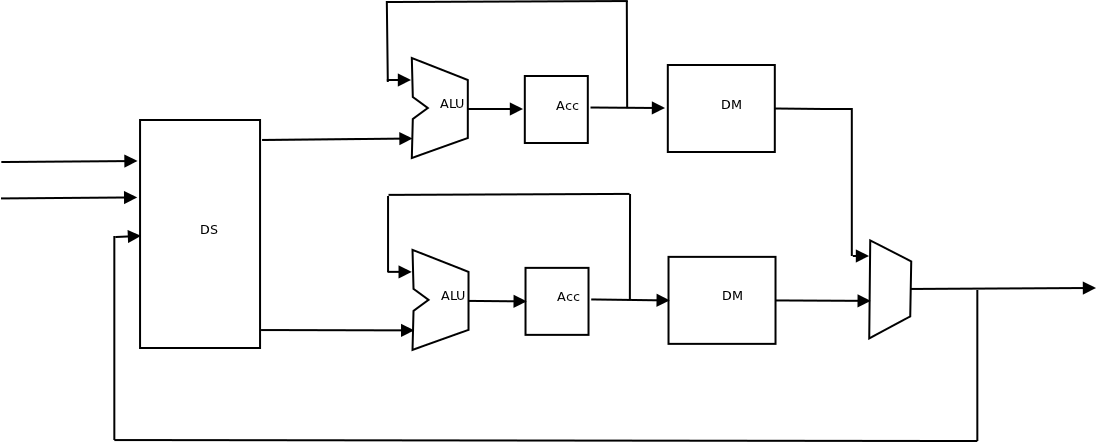
\includegraphics[width=0.8\textwidth]{images/new_path}
	\end{center}
	\caption{A block diagram of the modified area of the leros data path. ACC is the accumulator, DM is the data memory, DS is the data select.}
	\label{new_path}
\end{figure*}

The use of a 4 bit memory address operand limited the maximum number of additional ALUs to 32. A limit was also imposed by the board used as it only contained 36 blocks of ram meaning that even if a larger operand had been used little extra performance would be gained \cite{spartan_ram}. This meant that the board's memory was again acting as the bottleneck for the design as, with the exception of memory, the FPGA contained space to synthesise several hundred ALUs as was the original intent. The only option available at this point  to improve the memory was to use flip-flops instead of the ram. This was highly undesirable for two reasons. Firstly the number of flip-flops that were possible was only around 10,000 \cite{spartan_user}, while this may be more than enough for most applications, when being used as memory this was insufficient for the image processing operations around which the CPU was designed. Secondly, the use of flip-flops rather than the on-board memory meant that the maximum clock speed of the CPU was reduced by around 50\%. Because of these issues the implementation with a limit of 32 ALUs was kept.

The movement of data between memory blocks meant that while the CPU could perform the arithmetic and logical operations in parallel its memory operations could only occur in serial and due to the need to move data between memory blocks a significantly higher number of these load and store operations would be required for the program to perform. How much this affected the speed up of the additional ALUs would be largely program dependent. 

The implementation of several other instructions required alteration to work with the new multiple ALUs. The add and load immediate operations were altered to allow the immediate to be placed on the bus to all the ALUs so that they all performed the operation. All the branching and jumping operations operated only on the first ALU with this ALU being the only one  queried for branch conditionals This was done as with a single control unit the ALUs all had to perform the same instructions and so could not branch to different sections of code.


\subsection{Assembler for VHDL}

  Leros provided us with an assembler, based on an ANTLR (ANother Tool for
  Language Recognition) generated Java parser and lexer.  Because of the
  significant changes that would be required to add in support for vector
  operations, along with no one in the group having experience with ANTLR, it
  was decided that re-writing an assembler in a known language would be useful.

  The re-write was performed using Ruby; a two-pass assembler was created that
  matched the output of the Leros assembler, with one difference.  The
  Leros assembler output a VHDL file to be synthesised as a ROM, whereas the new assembler
  output a binary file.  To keep the integrated ROM a VHDLiser was also written
  that took the binary as input and output a VHDL ROM.
